% (find-LATEX "2022-1-C2-VSA.tex")
% (defun c () (interactive) (find-LATEXsh "lualatex -record 2022-1-C2-VSA.tex" :end))
% (defun C () (interactive) (find-LATEXsh "lualatex 2022-1-C2-VSA.tex" "Success!!!"))
% (defun D () (interactive) (find-pdf-page      "~/LATEX/2022-1-C2-VSA.pdf"))
% (defun d () (interactive) (find-pdftools-page "~/LATEX/2022-1-C2-VSA.pdf"))
% (defun e () (interactive) (find-LATEX "2022-1-C2-VSA.tex"))
% (defun o () (interactive) (find-LATEX "2022-1-C2-VSA.tex"))
% (defun u () (interactive) (find-latex-upload-links "2022-1-C2-VSA"))
% (defun v () (interactive) (find-2a '(e) '(d)))
% (defun d0 () (interactive) (find-ebuffer "2022-1-C2-VSA.pdf"))
% (defun cv () (interactive) (C) (ee-kill-this-buffer) (v) (g))
%          (code-eec-LATEX "2022-1-C2-VSA")
% (find-pdf-page   "~/LATEX/2022-1-C2-VSA.pdf")
% (find-sh0 "cp -v  ~/LATEX/2022-1-C2-VSA.pdf /tmp/")
% (find-sh0 "cp -v  ~/LATEX/2022-1-C2-VSA.pdf /tmp/pen/")
%     (find-xournalpp "/tmp/2022-1-C2-VSA.pdf")
%   file:///home/edrx/LATEX/2022-1-C2-VSA.pdf
%               file:///tmp/2022-1-C2-VSA.pdf
%           file:///tmp/pen/2022-1-C2-VSA.pdf
% http://angg.twu.net/LATEX/2022-1-C2-VSA.pdf
% (find-LATEX "2019.mk")
% (find-sh0 "cd ~/LUA/; cp -v Pict2e1.lua Pict2e1-1.lua Piecewise1.lua ~/LATEX/")
% (find-sh0 "cd ~/LUA/; cp -v Pict2e1.lua Pict2e1-1.lua Pict3D1.lua ~/LATEX/")
% (find-sh0 "cd ~/LUA/; cp -v C2Subst1.lua C2Formulas1.lua ~/LATEX/")
% (find-sh0 "cd ~/LUA/; cp -v Lazy5.lua Pict2e1.lua Verbatim1.lua ~/LATEX/")
% (find-CN-aula-links "2022-1-C2-VSA" "2" "c2m221vsa" "c2vs")

% «.defs»		(to "defs")
% «.defs-T-and-B»	(to "defs-T-and-B")
% «.title»		(to "title")
% «.questao-1»		(to "questao-1")
% «.questao-1-gab»	(to "questao-1-gab")
% «.questao-2»		(to "questao-2")
% «.questao-2-gab»	(to "questao-2-gab")
%
% «.djvuize»		(to "djvuize")



% <videos>
% Video (not yet):
% (find-ssr-links     "c2m221vsa" "2022-1-C2-VSA")
% (code-eevvideo      "c2m221vsa" "2022-1-C2-VSA")
% (code-eevlinksvideo "c2m221vsa" "2022-1-C2-VSA")
% (find-c2m221vsavideo "0:00")

\documentclass[oneside,12pt]{article}
\usepackage[colorlinks,citecolor=DarkRed,urlcolor=DarkRed]{hyperref} % (find-es "tex" "hyperref")
\usepackage{amsmath}
\usepackage{amsfonts}
\usepackage{amssymb}
\usepackage{pict2e}
\usepackage[x11names,svgnames]{xcolor} % (find-es "tex" "xcolor")
\usepackage{colorweb}                  % (find-es "tex" "colorweb")
%\usepackage{tikz}
%
% (find-dn6 "preamble6.lua" "preamble0")
%\usepackage{proof}   % For derivation trees ("%:" lines)
%\input diagxy        % For 2D diagrams ("%D" lines)
%\xyoption{curve}     % For the ".curve=" feature in 2D diagrams
%
\usepackage{edrx21}               % (find-LATEX "edrx21.sty")
\input edrxaccents.tex            % (find-LATEX "edrxaccents.tex")
\input edrx21chars.tex            % (find-LATEX "edrx21chars.tex")
\input edrxheadfoot.tex           % (find-LATEX "edrxheadfoot.tex")
\input edrxgac2.tex               % (find-LATEX "edrxgac2.tex")
%\usepackage{emaxima}              % (find-LATEX "emaxima.sty")
%
%\usepackage[backend=biber,
%   style=alphabetic]{biblatex}            % (find-es "tex" "biber")
%\addbibresource{catsem-slides.bib}        % (find-LATEX "catsem-slides.bib")
%
% (find-es "tex" "geometry")
\usepackage[a6paper, landscape,
            top=1.5cm, bottom=.25cm, left=1cm, right=1cm, includefoot
           ]{geometry}
%
\begin{document}

\catcode`\^^J=10
\directlua{dofile "dednat6load.lua"}  % (find-LATEX "dednat6load.lua")
%%L dofile "Piecewise1.lua"           -- (find-LATEX "Piecewise1.lua")
%%L dofile "QVis1.lua"                -- (find-LATEX "QVis1.lua")
%%L dofile "Pict3D1.lua"              -- (find-LATEX "Pict3D1.lua")
%%L dofile "C2Formulas1.lua"          -- (find-LATEX "C2Formulas1.lua")
%L dofile "Lazy5.lua"                -- (find-LATEX "Lazy5.lua")
%L dofile "2022-1-C2-P2.lua"         -- (find-LATEX "2022-1-C2-P2.lua")
%L Pict2e.__index.suffix = "%"
\pu
\def\pictgridstyle{\color{GrayPale}\linethickness{0.3pt}}
\def\pictaxesstyle{\linethickness{0.5pt}}
\def\pictnaxesstyle{\color{GrayPale}\linethickness{0.5pt}}
\celllower=2.5pt

% «defs»  (to ".defs")
% (find-LATEX "edrx21defs.tex" "colors")
% (find-LATEX "edrx21.sty")

\def\u#1{\par{\footnotesize \url{#1}}}

\def\drafturl{http://angg.twu.net/LATEX/2022-1-C2.pdf}
\def\drafturl{http://angg.twu.net/2022.1-C2.html}
\def\draftfooter{\tiny \href{\drafturl}{\jobname{}} \ColorBrown{\shorttoday{} \hours}}

% «defs-T-and-B»  (to ".defs-T-and-B")
% (c3m202p1p 6 "questao-2")
% (c3m202p1a   "questao-2")
\long\def\ColorOrange#1{{\color{orange!90!black}#1}}
\def\T(Total: #1 pts){{\bf(Total: #1)}}
\def\T(Total: #1 pts){{\bf(Total: #1 pts)}}
\def\T(Total: #1 pts){\ColorRed{\bf(Total: #1 pts)}}
\def\B       (#1 pts){\ColorOrange{\bf(#1 pts)}}

\def\eqnp      {\eqnpfull}
\def\lac       {▁▁}
\def\lac       {{\color{Red3}{▁}}}




%  _____ _ _   _                               
% |_   _(_) |_| | ___   _ __   __ _  __ _  ___ 
%   | | | | __| |/ _ \ | '_ \ / _` |/ _` |/ _ \
%   | | | | |_| |  __/ | |_) | (_| | (_| |  __/
%   |_| |_|\__|_|\___| | .__/ \__,_|\__, |\___|
%                      |_|          |___/      
%
% «title»  (to ".title")
% (c2m221vsap 1 "title")
% (c2m221vsaa   "title")

\thispagestyle{empty}

\begin{center}

\vspace*{1.2cm}

{\bf \Large Cálculo 2 - 2022.1}

\bsk

VS aberta (VSA)

\bsk

Eduardo Ochs - RCN/PURO/UFF

\url{http://angg.twu.net/2022.1-C2.html}

\end{center}

\newpage

%   ___                  _                _ 
%  / _ \ _   _  ___  ___| |_ __ _  ___   / |
% | | | | | | |/ _ \/ __| __/ _` |/ _ \  | |
% | |_| | |_| |  __/\__ \ || (_| | (_) | | |
%  \__\_\\__,_|\___||___/\__\__,_|\___/  |_|
%                                           
% «questao-1»  (to ".questao-1")
% (c2m221vsap 2 "questao-1")
% (c2m221vsaa   "questao-1")
% (find-angg ".emacs" "c2-2019-1")
% (find-angg ".emacs" "c2-2019-2")
% (c2m192p1p 4 "gabarito")
% (c2m192p1a   "gabarito")

%L ang("_", [[
%L   \begin{array}{rcll}
%L     <EDOLG_> &=& <EDOLG> \\
%L   \end{array}
%L ]]):sa("EDOLG="):output()
\pu

{\bf Questão 1}

\sa{[ECS]}{\CFname{ECS}{}}
\def\ECSn#1{\CFname{ECS}{_{#1}}}

\scalebox{0.42}{\def\colwidth{12.5cm}\firstcol{

\vspace*{-0.25cm}

\T(Total: 3.0 pts)

    Esta questão é continuação das questões sobre EDOs de 2a ordem
    (``lineares, com coeficientes constantes, etc, etc...'') que eu
    pus na P2 e na VR. Quando eu puser essa prova na página do curso
    eu vou colocar links pra essas questões.

    \msk

    Em todas as questões desta prova uma lacuna como $\lac$ quer dizer
    ``aqui vai ter um número mas eu não posso dizer qual é -- você vai
    ter que descobrir ele''... por exemplo, $e^{\lac x}$ pode ser
    $e^{42 x}$, $e^{-200 x}$, ou outras coisas assim.

\msk


Sejam:

\msk

$\ga{[ECS]} = \left(
 \begin{array}{rcl}
                     e^{iθ}  &=& \cos  θ + i\senθ\\
                     \sen -θ &=& -\sen θ \\
                     \cos -θ &=& -\cos θ \\
                     e^{-iθ} &=& \cos -θ + i\sen-θ\\
                             &=& \cos -θ - i\sen θ\\
                             &=& \cos  θ - i\sen θ\\
              e^{iθ}+e^{-iθ} &=& 2\cos θ \\
              e^{iθ}-e^{-iθ} &=& 2i\sen θ \\
              \cos θ & \eqnp{9}& \frac1 2  (e^{iθ} + e^{-iθ}) \\
              \sen θ &\eqnp{10}& \frac1{2i}(e^{iθ} - e^{-iθ}) \\
             \cos kθ &\eqnp{11}& \frac1 2  (e^{ikθ} + e^{-ikθ}) \\
             \sen kθ &\eqnp{12}& \frac1{2i}(e^{ikθ} - e^{-ikθ}) \\
   e^{(α+βi)θ} + e^{(α-βi)θ} &=& e^α (e^{βiθ} + e^{-βiθ}) \\
                             &=& 2 \, e^α \cos βθ \\
   e^{(α+βi)θ} - e^{(α-βi)θ} &=& e^α (e^{βiθ} - e^{-βiθ}) \\
                             &=& 2i \, e^α \cos βθ \\
 \end{array}
 \right)
$

\bsk

$\ga{EDOLG=}$



}\anothercol{

Eu vou usar notações como $\ECSn{9}$ e $\ECSn{13..14}$ pra me referir
a linhas individuais e a sequências contíguas de linhas do
$\ga{[ECS]}$.

Todas as linhas são fáceis de demonstrar a partir da $\ECSn{1}$, mas
muita gente tinha dificuldade em passar das igualdades (9) e (10) pras
(11) e (12), porque isso precisa de uma substituição como $[θ:=kθ]$.

A $\ECSn{1}$ é complicada de demonstrar -- nos semestres ``normais'' a
gente via uma introdução a séries de Taylor pra se convencer de que a
$\ECSn{1}$ é verdade, mas a gente não via uma demonstração formal da
$\ECSn{1}$.

\bsk

a) \B(0.2 pts) Calcule o resultado da substituição
%
$$\CFname{EDOLG}{} \bmat{α:=-2+10i \\ β:=-2-10i}
$$

e chame-o de $\CFname{E}{_1}$.

\bsk

b) \B(2.8 pts) As idéias da $\ga{[ECS]}$ devem indicar que existe uma
função da forma $g_1(x) = e^{\lac x} \cos(\lac x)$ que é solução da
EDO da primeira linha da resposta do seu item (a). Chame esta EDO de
$(*)$ e verifique se a sua função $g_1(x)$ é solução da EDO $(*)$. Se
não for chute outra função -- chame-a de $g_2(x)$ -- e veja se ela é
solução da EDO $(*)$. Se ainda não for faça outro chute-e-teste, e
repita. Lembre de NUNCA de apagar um chute-e-teste que não resolveu o
seu problema original.


}}

% (find-LATEX "2022-1-C2-P2.lua" "edo-2a-ordem")

\newpage

%   ___                  _                _               _     
%  / _ \ _   _  ___  ___| |_ __ _  ___   / |   __ _  __ _| |__  
% | | | | | | |/ _ \/ __| __/ _` |/ _ \  | |  / _` |/ _` | '_ \ 
% | |_| | |_| |  __/\__ \ || (_| | (_) | | | | (_| | (_| | |_) |
%  \__\_\\__,_|\___||___/\__\__,_|\___/  |_|  \__, |\__,_|_.__/ 
%                                             |___/             
%
% «questao-1-gab»  (to ".questao-1-gab")
% (c2m221vsap 3 "questao-1-gab")
% (c2m221vsaa   "questao-1-gab")

{\bf Questão 1: gabarito}

%L ang("_", [[
%L   \begin{array}{l}
%L     <EDOLG_> = <EDOLG> \\ \\[-5pt]
%L     <EVSA1_> = <EDOLG_><SVSA1> = \\ \\[-5pt]
%L     = <EVSA1> \\ \\[-5pt]
%L     = <EVSA2> \\
%L   \end{array}
%L ]]):sa("Questao 1a gab"):output()
\pu


\scalebox{0.42}{\def\colwidth{20cm}\firstcol{

\vspace*{0.0pt}

$\ga{Questao 1a gab}$

\msk

A última linha acima diz que $e^{2x}e^{-10ix}$ e $e^{2x}e^{10ix}$

são soluções da EDO $f''(x) -4f'(x) + 104f(x) = 0$. \quad $(*)$

Então $e^{2x}e^{-10ix} + e^{2x}e^{10ix} = e^{2x}(2 \cos 10x)$

também deve ser solução dessa EDO, e $e^{2x}\cos 10x$ também.

Sejam $g(x) = e^{2x} \cos 10x$ e $h(x) = e^{2x} \sen 10x$. Daí:
%
$$\begin{array}{rcl}
   g'(x) &=& 2g(x) - 10h(x) \\
   h'(x) &=& 2h(x) + 10g(x) \\
  g''(x) &=& -96g(x) - 40h(x) \\
  h''(x) &=& -96h(x) + 40g(x) \\
  g''(x) -4g'(x) + 104g(x) &=& (-96g(x) - 40h(x)) -4(2g(x) - 10h(x)) + 104g(x) \\
                           &=& 0 \\
  h''(x) -4h'(x) + 104h(x) &=& (-96h(x) + 40g(x)) -4(2h(x) + 10g(x)) + 104h(x) \\
                           &=& 0 \\
  \end{array}
$$

e portanto tanto $g(x)$ quanto $h(x)$ são soluções da EDO $(*)$.

% (setq eepitch-preprocess-regexp "^")
% (setq eepitch-preprocess-regexp "^%T ")
%
%T  (eepitch-maxima)
%T  (eepitch-kill)
%T  (eepitch-maxima)
%T g   : %e^(2*x) * cos(10*x);
%T h   : %e^(2*x) * sin(10*x);
%T gx  : diff(g,  x);
%T hx  : diff(h,  x);
%T gxx : diff(gx, x);
%T hxx : diff(hx, x);
%T expand(gxx - 4 * gx + 104 * g);
%T expand(hxx - 4 * hx + 104 * h);
%T gx - (2*g -10*h);
%T hx - (2*h +10*g);
%T gxx - (-96*g - 40*h);
%T hxx - (-96*h + 40*g);



}\anothercol{
}}


\newpage

%   ___                  _                ____  
%  / _ \ _   _  ___  ___| |_ __ _  ___   |___ \ 
% | | | | | | |/ _ \/ __| __/ _` |/ _ \    __) |
% | |_| | |_| |  __/\__ \ || (_| | (_) |  / __/ 
%  \__\_\\__,_|\___||___/\__\__,_|\___/  |_____|
%                                               
% «questao-2»  (to ".questao-2")
% (c2m221vsap 4 "questao-2")
% (c2m221vsaa   "questao-2")

{\bf Questão 2}

\def\TTT#1#2{
  \left(
  \begin{array}{rcl}
    \sqrt{#1^2 - #2^2x^2 \mathstrut}
      &=& \sqrt{#1^2 - \frac{#1^2}{#1^2} #2^2x^2} \\
      &=& \sqrt{#1^2 \left(1 - \frac{#2^2}{#1^2} x^2 \right)} \\
      &=& \sqrt{#1^2 \mathstrut} \, \sqrt{1 - \frac{#2^2}{#1^2} x^2} \\
      &=& #1 \, \sqrt{1 - \left(\frac{#2}{#1}x\right)^2} \\
  \end{array}
  \right)
  }

\scalebox{0.55}{\def\colwidth{10cm}\firstcol{

\vspace*{-0.25cm}

\T(Total: 7.0 pts)

Alguns livros ensinam substituição trigonométrica começando direto por
casos complicados em que o ``termo malvado'' da integral é este:
%
$$\sqrt{α^2 - β^2x^2}$$

Seja:
%
$$\CFname{T}{} = \TTT{α}{β}$$

a) \B(0.2 pts) Calcule:
%
$$\CFname{T}{} \bmat{α:=2 \\ β:=3}
$$

}\anothercol{

b) \B(2.8 pts) Digamos que a gente quer transformar esta integral
%
$$\intx{x^2\sqrt{4-9x^2}} \qquad (**)
$$

numa mais simples usando substituição trigonométrica. Use o truque do
item (a), o $\CFname{MV}{_2}$ e as idéias do gabarito da questão 1 da
P2 pra transformar a $(**)$ em ``algo em $θ$''.

\msk

c) \B(4.0 pts) Digamos que $({*}{*}{*})$ é esta integral:
%
$$\intx{x^γ\sqrt{α^2-β^2x^2}^δ} \qquad ({*}{*}{*})
$$

Mostre que uma mudança de variável com $u=\frac{β}{α}x$ transforma
esta integral numa da forma:
%
$$\lac \intx{u^{\lac} \left(\sqrt{1-u^2}\right)^{\lac}}
$$

Dica: comece com o caso particular em que $γ=1$ e $δ=1$ e depois tente
casos mais complicados.

\msk

{\sl Peçam dicas!!!}

}}

\newpage

%   ___                  _                ____                _     
%  / _ \ _   _  ___  ___| |_ __ _  ___   |___ \    __ _  __ _| |__  
% | | | | | | |/ _ \/ __| __/ _` |/ _ \    __) |  / _` |/ _` | '_ \ 
% | |_| | |_| |  __/\__ \ || (_| | (_) |  / __/  | (_| | (_| | |_) |
%  \__\_\\__,_|\___||___/\__\__,_|\___/  |_____|  \__, |\__,_|_.__/ 
%                                                 |___/             
% «questao-2-gab»  (to ".questao-2-gab")
% (c2m221vsap 5 "questao-2-gab")
% (c2m221vsaa   "questao-2-gab")

{\bf Questão 2: gabarito}


\scalebox{0.6}{\def\colwidth{15cm}\firstcol{

a) $\CFname{T}{} \bmat{α:=2 \\ β:=3} \;=\; \TTT{2}{3}$

b) $\begin{array}{rcl}
     \intx{x^2 \sqrt{4-9x^2}}
       &=& \intx{x^2 \sqrt{2^2-3^2x^2}} \\
       &=& \intx{x^2 · 2\sqrt{1-(\frac32 x)^2}} \\
       &=& \intu{(\frac23u)^2 · 2\sqrt{1-u^2}·\frac23} \\
       &=& \intu{(\frac23)^3·2· u^2\sqrt{1-u^2}} \\
       &=& \frac{16}{27} \intu{u^2\sqrt{1-u^2}} \\
       &=& \frac{16}{27} \intth{(\senθ)^2\sqrt{1-(\senθ)^2}·\cosθ} \\
       &=& \frac{16}{27} \intth{(\senθ)^2\sqrt{(\cosθ)^2}·\cosθ} \\
       &=& \frac{16}{27} \intth{(\senθ)^2\cosθ·\cosθ} \\
       &=& \frac{16}{27} \intth{(\senθ)^2 (\cosθ)^2} \\
     \end{array}
   $
   \qquad
   $\begin{array}{c}
    \bsm{ u=\frac32x \\
          x=\frac23u \\
          du=\frac32dx \\
          dx=\frac23du
        }
    \\ \\
    \bsm{
      u = \senθ \\
      \frac{du}{dθ} = \cosθ \\
      du = \cosθ\,dθ \\
    }
    \end{array}
   $

}\anothercol{

}}


\newpage


{\bf Questão 2: gabarito (cont.)}

\scalebox{0.6}{\def\colwidth{15cm}\firstcol{

c) $\begin{array}{rcl}
      \intx{x^γ\sqrt{α^2-β^2x^2}^δ}
      &=& \intx{x^γ\sqrt{α^2(1-\frac{β^2}{α^2}x^2)}^δ} \\
      &=& \intx{x^γ\left(\sqrt{α^2(1-(\frac{β}{α}x)^2)}\right)^δ} \\
      &=& \intx{x^γ\left(α\sqrt{(1-(\frac{β}{α}x)^2)}\right)^δ} \\
      &=& α^γ \intx{x^γ\left(\sqrt{(1-(\frac{β}{α}x)^2)}\right)^δ} \\
      &=& α^γ \intu{(\fracαβ u)^γ\left(\sqrt{(1-u^2)}\right)^δ · \fracαβ} \\
      &=& α^γ (\fracαβ)^{γ+1} \intu{u^γ \sqrt{(1-u^2)}^δ} \\
    \end{array}
   $
   \qquad
   $\begin{array}{c}
    \bmat{ u=\fracβα x \\
          x=\fracαβ u \\
          du=\fracβα dx \\
          dx=\fracαβ du
        }
    \end{array}
   $

}\anothercol{
}}








\newpage

\hspace*{-1cm}
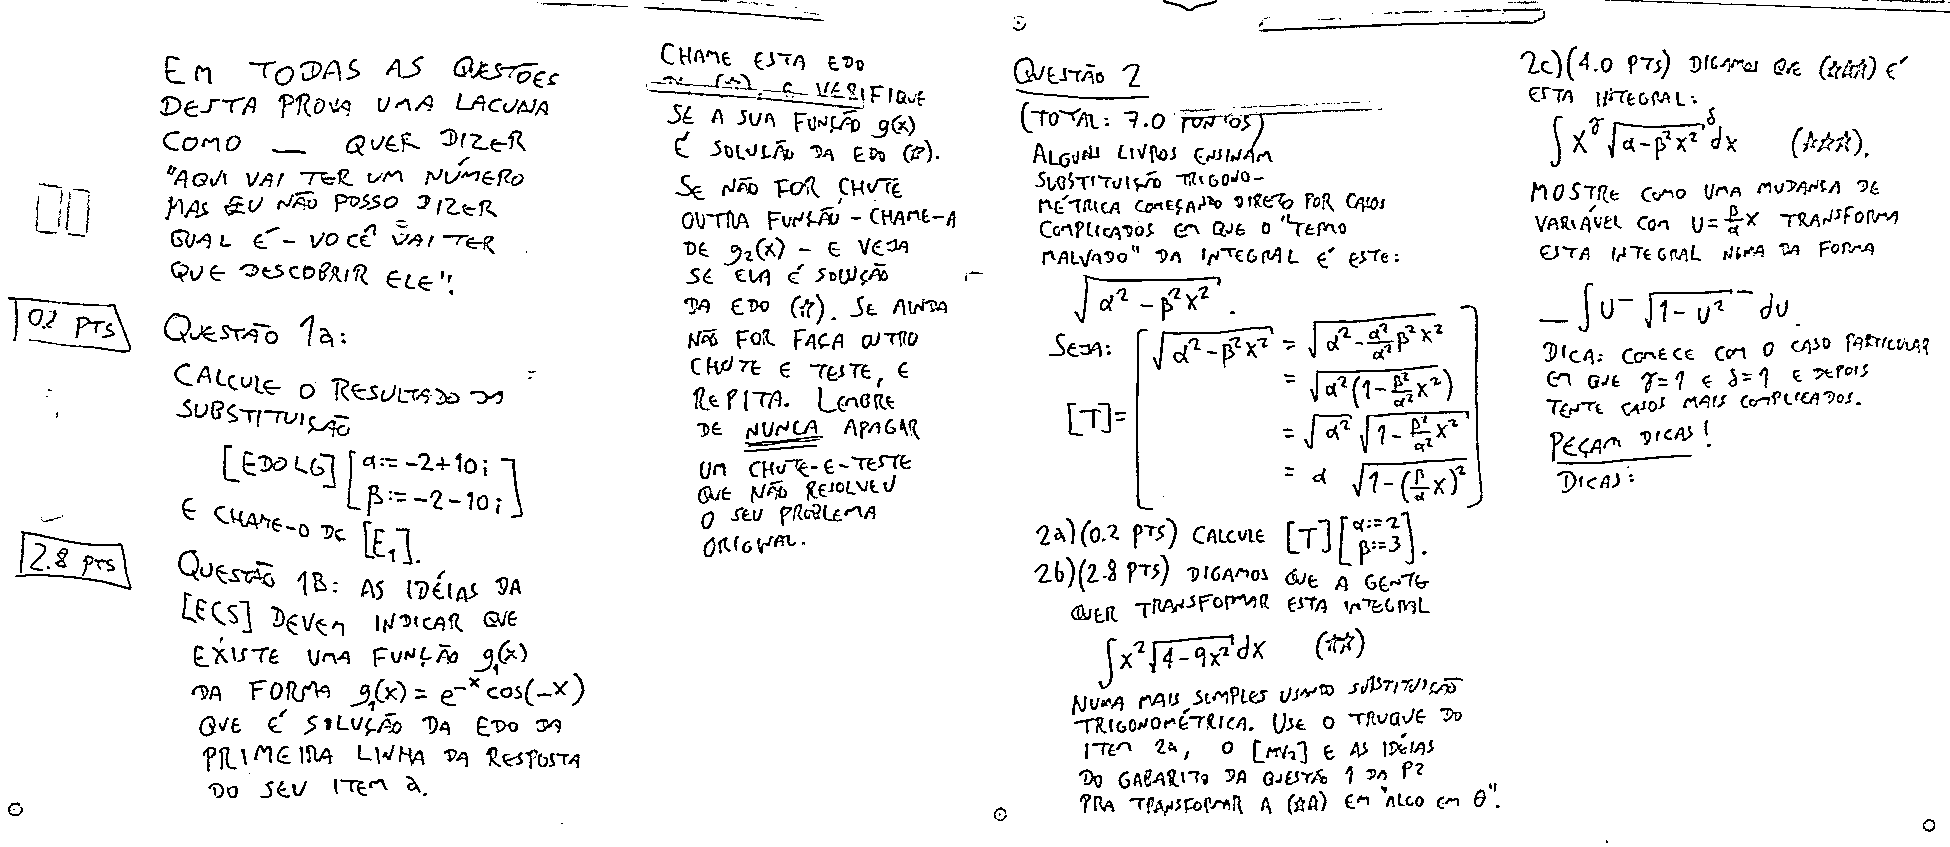
\includegraphics[width=13cm]{2022-1-C2/C2-VSA.pdf}

{\footnotesize

($↑$ Vou digitar isso aqui depois!)

}

\newpage

% (c2m221p2p 7 "subst-trig-gab")
% (c2m221p2a   "subst-trig-gab")

{\bf Gabarito da questão 1 da P2}

{\footnotesize (Com vários chutes e testes -- pra questão 2)}

% (find-LATEX "2022-1-C2-P2.lua" "subst-trig")
%L TRIGSOLUTION:sa("TRIGSOLUTION"):output()
\pu

\bsk

$\scalebox{0.6}{$\ga{TRIGSOLUTION}$}$



%\printbibliography

\GenericWarning{Success:}{Success!!!}  % Used by `M-x cv'

\end{document}

%  ____  _             _         
% |  _ \(_)_   ___   _(_)_______ 
% | | | | \ \ / / | | | |_  / _ \
% | |_| | |\ V /| |_| | |/ /  __/
% |____// | \_/  \__,_|_/___\___|
%     |__/                       
%
% «djvuize»  (to ".djvuize")
% (find-LATEXgrep "grep --color -nH --null -e djvuize 2020-1*.tex")




%  __  __       _        
% |  \/  | __ _| | _____ 
% | |\/| |/ _` | |/ / _ \
% | |  | | (_| |   <  __/
% |_|  |_|\__,_|_|\_\___|
%                        
% <make>

 (eepitch-shell)
 (eepitch-kill)
 (eepitch-shell)
# (find-LATEXfile "2019planar-has-1.mk")
make -f 2019.mk STEM=2022-1-C2-VSA veryclean
make -f 2019.mk STEM=2022-1-C2-VSA pdf

% Local Variables:
% coding: utf-8-unix
% ee-tla: "c2vs"
% ee-tla: "c2m221vsa"
% End:
